\documentclass[conference]{IEEEtran}
\IEEEoverridecommandlockouts
\usepackage{cite}
\usepackage{amsmath,amssymb,amsfonts}
\usepackage{graphicx}
\usepackage{textcomp}
\usepackage{xcolor}
\usepackage{booktabs}
\usepackage{courier}
\usepackage{tikz}
\usetikzlibrary{arrows.meta,positioning,shapes.misc}
\usepackage[hidelinks]{hyperref}
\newcommand{\AccA}{0.986}
\newcommand{\AccB}{0.975}
\newcommand{\AccC}{0.975}
\newcommand{\AdasynBefore}{3.26}
\newcommand{\AdasynDelta}{$-$0.002}
\newcommand{\AdasynDeltaSd}{0.015}
\newcommand{\AdasynRows}{950}
\newcommand{\AdasynSynth}{455}
\newcommand{\AdasynWins}{14}
\newcommand{\CkEpochWord}{the first}
\newcommand{\CkValScore}{1.000}
\newcommand{\CkptBytes}{132{,}009{,}232}
\newcommand{\CkptKb}{14}
\newcommand{\CkptMb}{132}
\newcommand{\ConcExpFour}{3.54}
\newcommand{\ConcExpOne}{3.61}
\newcommand{\ConcPredFour}{9.4}
\newcommand{\ConcPredOne}{9.4}
\newcommand{\ConfAcc}{0.986}
\newcommand{\ConfCorrect}{0.92}
\newcommand{\ConfMean}{0.918}
\newcommand{\ConfMedian}{0.945}
\newcommand{\ConfWrong}{0.73}
\newcommand{\CpuCount}{4}
\newcommand{\EOneAcc}{0.9535}
\newcommand{\EOneAccHi}{1.000}
\newcommand{\EOneAccLo}{0.884}
\newcommand{\EOneCmMatches}{identical to}
\newcommand{\EOneEarly}{0.960}
\newcommand{\EOneEarlyLo}{0.870}
\newcommand{\EOneEce}{0.104}
\newcommand{\EOneFone}{0.9653}
\newcommand{\EOneImpaired}{25}
\newcommand{\EOneKappa}{0.9783}
\newcommand{\EOneMissed}{1}
\newcommand{\EOneN}{43}
\newcommand{\EValN}{43}
\newcommand{\ExpPerS}{3.6}
\newcommand{\ExplainMedian}{293}
\newcommand{\ExplainPNinetyFive}{344}
\newcommand{\ExplainRatio}{2.6}
\newcommand{\FastapiVer}{0.162.0}
\newcommand{\FoneA}{0.987}
\newcommand{\FoneB}{0.975}
\newcommand{\FoneC}{0.971}
\newcommand{\GcCorrect}{0.774}
\newcommand{\GcFlag}{0}
\newcommand{\GcMean}{0.775}
\newcommand{\GcMedian}{0.701}
\newcommand{\GcMin}{0.587}
\newcommand{\GcN}{710}
\newcommand{\GcNWrong}{14}
\newcommand{\GcNWrongPct}{2.0}
\newcommand{\GcPfive}{0.645}
\newcommand{\GcWrongMean}{0.826}
\newcommand{\HttpExpOverhead}{1}
\newcommand{\HttpExplainMedian}{294}
\newcommand{\HttpHealthMedian}{2.17}
\newcommand{\HttpHwMedian}{11.8}
\newcommand{\HttpPredOverhead}{12}
\newcommand{\HttpPredictMedian}{123}
\newcommand{\HwAcc}{0.893}
\newcommand{\HwAccHi}{0.918}
\newcommand{\HwAccLo}{0.868}
\newcommand{\HwAnalyzeMedian}{10.0}
\newcommand{\HwAnalyzePNinetyFive}{16.5}
\newcommand{\HwAuc}{0.962}
\newcommand{\HwAucHi}{0.975}
\newcommand{\HwAucLo}{0.946}
\newcommand{\HwBestSingle}{0.939}
\newcommand{\HwCvAcc}{0.923}
\newcommand{\HwCvAuc}{0.975}
\newcommand{\HwFeatMedian}{6.47}
\newcommand{\HwGbAcc}{0.882}
\newcommand{\HwGbAuc}{0.955}
\newcommand{\HwHeldN}{600}
\newcommand{\HwImpHigh}{82}
\newcommand{\HwImpLow}{6}
\newcommand{\HwJsonKb}{21.9}
\newcommand{\HwLoadMs}{1.75}
\newcommand{\HwMaxDrop}{0.004}
\newcommand{\HwMaxDropName}{tremor}
\newcommand{\HwModShare}{14}
\newcommand{\HwNoiseFourAcc}{0.648}
\newcommand{\HwNoiseFourAuc}{0.928}
\newcommand{\HwNoiseTwoAcc}{0.862}
\newcommand{\HwPoints}{982}
\newcommand{\HwRho}{0.969}
\newcommand{\HwScaleMax}{6.8\times10^{-14}}
\newcommand{\HwSens}{0.890}
\newcommand{\HwSpec}{0.897}
\newcommand{\HwTrainN}{600}
\newcommand{\HwTrainS}{5.7}
\newcommand{\HwTypHigh}{3}
\newcommand{\HwTypLow}{81}
\newcommand{\ImpRows}{950}
\newcommand{\LocFront}{1,433}
\newcommand{\LocScripts}{1,310}
\newcommand{\LocSrc}{2,625}
\newcommand{\LocTests}{684}
\newcommand{\ModelLoadS}{1.7}
\newcommand{\MpFourKb}{766}
\newcommand{\ParamsTotalM}{33.0}
\newcommand{\ParamsTrainM}{22.4}
\newcommand{\PngKb}{32.6}
\newcommand{\PoolAcc}{0.978}
\newcommand{\PoolAccHi}{0.987}
\newcommand{\PoolAccLo}{0.969}
\newcommand{\PoolAdjErr}{23}
\newcommand{\PoolAuc}{0.998}
\newcommand{\PoolBal}{0.979}
\newcommand{\PoolBrier}{0.051}
\newcommand{\PoolEarly}{0.992}
\newcommand{\PoolEce}{0.060}
\newcommand{\PoolEmciLmci}{14}
\newcommand{\PoolEmciNc}{5}
\newcommand{\PoolEmciRecall}{0.931}
\newcommand{\PoolFarErr}{0}
\newcommand{\PoolFone}{0.978}
\newcommand{\PoolFoneHi}{0.986}
\newcommand{\PoolFoneLo}{0.968}
\newcommand{\PoolImpaired}{615}
\newcommand{\PoolKappa}{0.990}
\newcommand{\PoolLmciPrec}{0.931}
\newcommand{\PoolMissedImpaired}{5}
\newcommand{\PoolN}{1,065}
\newcommand{\PoolNll}{0.122}
\newcommand{\PoolWrong}{23}
\newcommand{\PredPerS}{9.4}
\newcommand{\PredictMedian}{111}
\newcommand{\PredictPNinetyFive}{150}
\newcommand{\PreprocMedian}{0.28}
\newcommand{\PyVer}{3.13.17}
\newcommand{\RamGb}{16}
\newcommand{\RobBlurE}{0.976}
\newcommand{\RobBlurF}{0.822}
\newcommand{\RobBrightE}{0.888}
\newcommand{\RobBrightF}{0.942}
\newcommand{\RobCleanE}{0.995}
\newcommand{\RobCleanF}{0.987}
\newcommand{\RobContrastE}{0.898}
\newcommand{\RobContrastF}{0.947}
\newcommand{\RobJpegE}{0.922}
\newcommand{\RobJpegF}{0.807}
\newcommand{\RobNoiseFiveE}{1.000}
\newcommand{\RobNoiseFiveF}{0.919}
\newcommand{\RobNoiseTenE}{1.000}
\newcommand{\RobNoiseTenF}{0.648}
\newcommand{\RobNoiseTwentyE}{1.000}
\newcommand{\RobNoiseTwentyF}{0.443}
\newcommand{\RobRotateE}{0.980}
\newcommand{\RobRotateF}{0.965}
\newcommand{\RobShiftE}{0.995}
\newcommand{\RobShiftF}{0.968}
\newcommand{\RssAfterExplain}{319}
\newcommand{\RssAfterLoad}{138}
\newcommand{\SciVer}{1.18.1}
\newcommand{\ServerColdS}{11.6}
\newcommand{\ServerRssMb}{1,183}
\newcommand{\SklVer}{1.9.1}
\newcommand{\StaticNoVideoKb}{182}
\newcommand{\StaticTotalKb}{1,665}
\newcommand{\TestCount}{88}
\newcommand{\TestSeconds}{42}
\newcommand{\ThroughputBatchOne}{9.1}
\newcommand{\ThroughputBatchSixteen}{7.5}
\newcommand{\TorchThreads}{4}
\newcommand{\TorchVer}{2.14.1+cu130}
\newcommand{\UvicornVer}{0.54.0}
\newcommand{\WebmKb}{710}


\begin{document}

\title{Early Detection of Alzheimer's Disease from MRI and Handwriting: Design and Analysis of an Explainable Multimodal Prototype}

\author{Sathwik Hejamady Bhat, Malhar Srivatsav,\\
Harit Raval, Parthav Udayasankar,\\
Kushith Reddy}

\maketitle

\begin{abstract}
This report documents an explainable prototype for the early detection of Alzheimer's disease and evaluates its latest revision. The system classifies a two-dimensional MRI slice into four ordered stages (normal cognition, early and late mild cognitive impairment, and Alzheimer's disease) with a fine-tuned VGG19 network, and it explains each prediction with a Grad-CAM attribution map and an automatic check of where that map falls. A second module scores a spiral drawing captured in the browser from the timestamped pen trace, using nine kinematic features and a logistic regression whose output decomposes exactly into per-feature contributions. Clinical records are completed with hot-deck imputation and balanced with ADASYN. Everything is served by a FastAPI application and a single-page interface. All data in this work are synthetic: the MRI slices are generated phantoms and the drawings are simulated, so every accuracy figure describes the pipeline and the generator and not patients. Executing the released checkpoint reproduces the reported test split exactly (\EOneN{} slices, accuracy \EOneAcc{}, macro F1 \EOneFone{}) and reaches accuracy \PoolAcc{} and macro F1 \PoolFone{} on \PoolN{} slices from three freshly generated cohorts, with expected calibration error \PoolEce{}. The handwriting classifier reaches AUC \HwAuc{} on \HwHeldN{} held-out drawings, and its ranking, but not its decision threshold, survives heavy coordinate noise. Hot-deck imputation preserves variance where mean imputation removes it, whereas ADASYN gives no measurable downstream gain on the synthetic table. Median CPU latency is \PredictMedian{} ms for a prediction and \ExplainMedian{} ms for a prediction with explanation. The report separates measured results from derived quantities and from claims it does not make, and it lists the steps required before any clinical interpretation.
\end{abstract}

\begin{IEEEkeywords}
Alzheimer's disease, MRI classification, Grad-CAM, transfer learning, handwriting analysis, hot-deck imputation, ADASYN, FastAPI.
\end{IEEEkeywords}

\section{Introduction}
Alzheimer's disease advances through recognizable stages, from normal cognition through early and late mild cognitive impairment to dementia, and the Alzheimer's Disease Neuroimaging Initiative organizes its data around that progression \cite{adni}. Structural MRI shows the change as enlarged ventricles, thinner cortex, and a shrinking hippocampus, but early differences are subtle, and a network that reports only a label gives a reviewer nothing to check. The project examined here, whose source repository is \cite{repo}, pairs a stage classifier with an attribution map that shows where the evidence lies and adds handwriting as a second, inexpensive signal.

The central requirement is that every reported number stay attributable to what it measures. The repository contains no ADNI images or handwriting recordings: its MRI slices are phantoms drawn by a generator and its drawings come from a simulator. A high score on such data shows that the pipeline is connected correctly and that the generator is separable, not that the model detects disease. This report therefore separates measurements produced by executing the repository, quantities derived from code and constants, and claims it does not make.

The report has four objectives. First, it describes the system precisely enough to reproduce it. Second, it reproduces the figures reported by the repository authors and measures the released checkpoint on unseen cohorts, including calibration, robustness, explanation focus, and latency. Third, it isolates the contribution of the imputation and balancing stages and of the handwriting features. Fourth, it states the limits of the evidence and orders the work needed before any clinical interpretation.

\section{Background and Design Context}
\subsection{Staging Task and Ordinal Structure}
The four classes are ordered: NC $<$ EMCI $<$ LMCI $<$ AD. Calling an Alzheimer's case normal is a more serious error than confusing the two mild stages, so accuracy alone is a weak headline metric, particularly when about 42\% of a cohort is normal. The implementation therefore reports macro F1, balanced accuracy, quadratic-weighted kappa \cite{kappa}, and the fraction of impaired cases that are not called normal (Section~\ref{sec:method}).

\subsection{Transfer Learning and Explanation}
VGG19 \cite{vgg} pretrained on ImageNet \cite{imagenet} supplies the backbone. With a few hundred training slices there is no prospect of fitting its 143 million ImageNet-head parameters from scratch, but the early filters already respond to the edges and textures that ventricular enlargement and cortical thinning produce. VGG is also convenient for explanation: Grad-CAM \cite{gradcam} needs only the activations and gradients of a late convolutional layer, and VGG19 exposes one without architectural change.

\subsection{Handwriting as a Second Signal}
Kinematic studies of handwriting report group differences between healthy controls, people with mild cognitive impairment, and people with mild Alzheimer's disease. In one such study, temporal measures grew and pen pressure fell with greater decline, and kinematic plus cognitive variables classified 69\% to 72\% of participants correctly, with the intermediate group classified least well \cite{werner}. The DARWIN dataset provides 174 participants (89 with Alzheimer's disease and 85 healthy) who each performed 25 tasks on a graphic tablet \cite{darwin}. These sources motivate the choice of measurements; they do not validate the specific features or thresholds used here, and no recording from either source was used.

\subsection{Missing Data and Imbalance}
Clinical tables are incomplete, and here the missingness rises with stage, so deleting incomplete rows would remove the most impaired subjects first. Hot-deck imputation fills each gap with an observed value from a similar complete record \cite{hotdeck}, and ADASYN generates synthetic minority samples with emphasis on difficult neighbourhoods \cite{adasyn}. Both act on tabular records and never on images, because interpolating between two MRI slices produces anatomy that does not exist.

\subsection{System Requirements}
The functional requirements are image upload and four-stage classification, an explanation for each result, imputation and balancing of clinical records, capture and scoring of a spiral drawing, and a browser interface that needs no command-line interaction. The quality requirements are reproducibility, honest reporting of what the data can support, bounded request sizes, and graceful behaviour when no model is available. The repository meets these in part. It has request-size limits, typed error responses, and a health endpoint that reports whether a checkpoint is loaded. It has no authentication, persistent storage, audit log, or subject-level data handling, and these are absent capabilities and not defects of the implemented ones.

\section{System Architecture}
\subsection{Layered Organization}
Figure~\ref{fig:layers} summarizes the request path. The browser submits an image or a timestamped stroke list to a FastAPI application. The application validates sizes and content, then calls the MRI predictor or the handwriting analyzer. Both return structured results, and the interface renders them together with the explanation. The training and data-preparation stages run offline from command-line modules and are connected to serving only through the checkpoint file.

\begin{figure}[t]
\centering
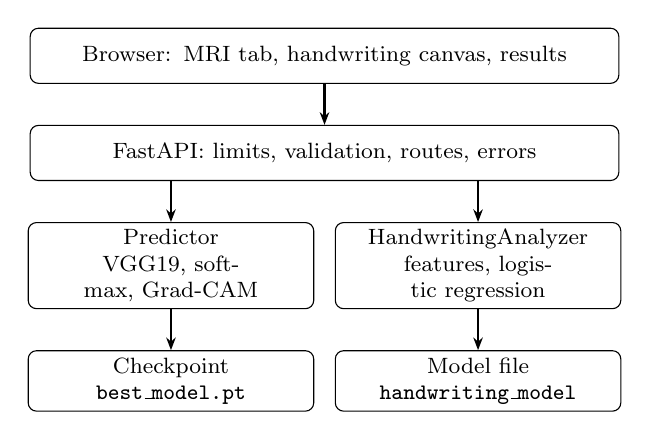
\begin{tikzpicture}[
  node distance=5.2mm,
  box/.style={draw, rounded corners=3pt, minimum height=7mm, align=center, font=\footnotesize, inner sep=2.5pt},
  wide/.style={box, text width=7.3cm},
  half/.style={box, text width=3.45cm},
  arr/.style={-{Stealth[length=1.6mm]}, thick}]
  \node[wide] (ui) {Browser: MRI tab, handwriting canvas, results};
  \node[wide, below=of ui] (api) {FastAPI: limits, validation, routes, errors};
  \node[half, below=of api, xshift=-1.95cm] (mri) {Predictor\\VGG19, softmax, Grad-CAM};
  \node[half, below=of api, xshift=1.95cm] (hw) {HandwritingAnalyzer\\features, logistic regression};
  \node[half, below=of mri] (ck) {Checkpoint\\\texttt{best\_model.pt}};
  \node[half, below=of hw] (jb) {Model file\\\texttt{handwriting\_model}};
  \draw[arr] (ui) -- (api);
  \draw[arr] (api.south) ++(-1.95cm,0) -- (mri.north);
  \draw[arr] (api.south) ++(1.95cm,0) -- (hw.north);
  \draw[arr] (mri) -- (ck);
  \draw[arr] (hw) -- (jb);
\end{tikzpicture}
\caption{Logical layers of the prototype. The two modalities are served by separate analyzers behind one API. The only coupling between them is an illustrative average computed in the browser (Section~\ref{sec:fusion}).}
\label{fig:layers}
\end{figure}

\subsection{Component Responsibilities}
\texttt{data/imputation.py} implements the hot-deck imputer, and \texttt{data/balancing.py} implements ADASYN directly on \texttt{sklearn.neighbors}, so the project carries no resampling dependency. \texttt{data/datasets.py} builds manifests, stratified splits, transforms, and class weights. \texttt{models/vgg19.py} constructs the network and its checkpoint format, and \texttt{models/gradcam.py} computes the attribution map and its focus summary. \texttt{training/} contains the training loop and the ordinal-aware metrics. \texttt{inference.py} defines the \texttt{Predictor} shared by the API and the optional Streamlit dashboard, so the two surfaces cannot disagree. \texttt{handwriting/} contains feature extraction, the simulator, and the classifier. \texttt{api/main.py} defines the routes, and \texttt{api/static/} holds the interface.

\subsection{Implementation Stack}
The benchmarks in this report ran on Python \PyVer{} with PyTorch \TorchVer{} \cite{pytorch}, scikit-learn \SklVer{} \cite{sklearn}, SciPy \SciVer{} \cite{scipy}, FastAPI \FastapiVer{}, and Uvicorn \UvicornVer{}, on a CPU-only machine. These versions describe the measured environment. The project declares only lower bounds, so a reproduction should record the versions it actually resolves.

\subsection{Interface}
The interface is a single static page with no build step. The MRI tab offers an upload zone, labelled samples, a draggable comparison slider between scan and attribution, per-stage probabilities, and the attention audit. The handwriting tab offers a drawing canvas, replay of simulated drawings, a speed-coloured trace, and a feature-contribution chart. Its theme follows a shadcn/ui preset \cite{shadcn} (mauve tokens, small radius, Noto Sans body text, Playfair Display headings) with locally served fonts, and a looping video behind translucent panels is disabled when the viewer requests reduced motion.

\section{Data and Preprocessing}
\subsection{Synthetic Cohort}
The generator draws axial phantoms whose ventricle size, cortical thickness, and hippocampal scale change with stage, together with a clinical table of age, MMSE, CDR, ADAS-Cog, hippocampal volume, APOE4 status, and CSF amyloid. Table~\ref{tab:profile} lists the stage profile; the cohort shares give a class imbalance of about 3.2 to 1. Requesting 120 slices for the largest class gives 285 slices (NC 120, EMCI 74, LMCI 54, AD 37), the cohort on which the released checkpoint was trained, and requesting 150 gives 355 (150, 92, 67, 46). Missingness is highest in CSF amyloid and rises with stage.

\begin{table}[t]
\centering
\caption{Phantom Generator Profile by Stage (Derived from Code Constants)}
\label{tab:profile}
\begin{tabular}{@{}lccc@{}}
\toprule
Stage & Ventricle scale & Cortex thickness & Hippocampus \\
\midrule
NC   & 0.16 & 0.085 & 1.00 \\
EMCI & 0.21 & 0.072 & 0.90 \\
LMCI & 0.27 & 0.058 & 0.78 \\
AD   & 0.35 & 0.044 & 0.62 \\
\bottomrule
\end{tabular}
\end{table}

\subsection{Hot-Deck Imputation}
The imputer fits on complete training records. For a record with missing entries it standardizes the observed columns, finds the $k$ nearest complete donors by Euclidean distance on those columns, and copies the missing values from one donor chosen uniformly among them. Choosing among $k=5$ donors, not always the nearest, stops one donor from being copied into many recipients and collapsing the imputed variance. In training the pool is restricted to the record's own class, so an AD record never inherits a healthy control's hippocampal volume; at inference the label is unavailable and the global pool is used. A class with fewer than $k$ complete records also falls back to the global pool.

\subsection{ADASYN}
Let $m_l$ and $m_s$ be the majority and minority class counts. For each minority point $x_i$, the implementation counts $\Delta_i$ of its $K$ nearest neighbours in the full set that belong to another class, and sets
\begin{equation}
r_i = \frac{\Delta_i}{K}, \qquad \hat r_i = \frac{r_i}{\sum_j r_j}, \qquad g_i = \hat r_i\, G,
\label{eq:adasyn}
\end{equation}
with $G=(m_l-m_s)\beta$ synthetic samples to allocate across the class (largest-remainder rounding). Each synthetic point is $s = x_i + \lambda (x_{z_i}-x_i)$ with $\lambda\sim U(0,1)$ and $x_{z_i}$ a same-class neighbour. The original method counts majority-class neighbours \cite{adasyn}; this implementation counts neighbours of any other class, which coincides for two classes and is a reasonable generalization for four. A class with a single member is skipped. The setting $\beta=1$ balances every minority class to the majority count.

\subsection{Splits and Leakage Controls}
The image manifest is split into stratified 70/15/15 train, validation, and test partitions with seed 42. In the tabular stage the split precedes imputation, the imputer is fitted on training rows only, held-out rows are imputed but never resampled, and ADASYN is applied to the imputed training rows alone. Resampling a held-out partition would score the model against synthetic rows it has effectively seen. The split is by slice. The generator emits one slice per subject, so this equals a subject-level split here, but real data with several slices per subject would leak identity across partitions unless grouped by subject.

\section{Model and Training}
\subsection{Architecture}
The network is torchvision's VGG19 with every in-place ReLU replaced by an out-of-place one, because in-place activations overwrite the values Grad-CAM must read. The 1000-way ImageNet classifier is replaced by $25088\rightarrow512\rightarrow256\rightarrow4$ with dropout 0.5 and 0.25. All convolutional layers are frozen except the last block. The loaded model has \ParamsTotalM{} M parameters, of which \ParamsTrainM{} M are trainable under that freezing rule. Inputs are resized to $224\times224$ and normalized with ImageNet statistics.

\subsection{Training Procedure}
The recipe uses AdamW with learning rate $10^{-4}$ for the backbone and ten times that for the new head, weight decay $10^{-4}$, label smoothing 0.05, cosine decay over at most 25 epochs, and inverse-frequency class weights in the loss. Augmentation is deliberately mild (horizontal flip with probability 0.5, rotation up to $7^\circ$, translation up to 3\%, and 10\% brightness and contrast jitter), because slices are already registered and strong warping removes the atrophy cues. The checkpoint with the best validation macro F1 is kept, with early stopping after six epochs without gain.

\subsection{Checkpoint Under Test}
This report did not retrain the network. It evaluates the checkpoint released by the repository authors, whose metadata record the class list, a hidden width of 512, dropout 0.5, one trainable block, \CkEpochWord{} selected epoch, and a validation macro F1 of \CkValScore{}. Selecting the first epoch at a validation score of 1.0 shows that the validation partition (\EValN{} slices) is saturated: every later epoch could at best tie, so model selection on it carries no information. This is a property of the synthetic data and is discussed in Section~\ref{sec:limits}.

\section{Explanation and Attention Audit}
For class $c$, Grad-CAM weights each feature map $A^k$ of the target layer by the spatially averaged gradient of the class score $y^c$ and keeps the positive part,
\begin{equation}
\alpha^c_k = \frac{1}{Z}\sum_{u,v}\frac{\partial y^c}{\partial A^k_{uv}}, \qquad
L^c = \mathrm{ReLU}\!\Big(\sum_k \alpha^c_k A^k\Big).
\label{eq:gradcam}
\end{equation}
The target layer is \texttt{features.35}, the activation after the last convolution. Pointing at the preceding convolution output feeds the method values that swing negative, and the final ReLU then flattens every map to zero, a silent failure that a regression test pins. The $14\times14$ map is upsampled to $224\times224$ and min-max normalized, with a dead map returned as zeros. A request may ask for any class, which supports the counterfactual question of what would have made a scan read as AD.

The attention audit summarizes where the map falls. With $L$ normalized to $[0,1]$, the central share is
\begin{equation}
S = \frac{\sum_{(u,v)\in \mathcal{C}} L_{uv}}{\sum_{u,v} L_{uv}},
\label{eq:central}
\end{equation}
where $\mathcal{C}$ is the central half of the frame in each dimension. The interface flags a prediction as unverified when $S<0.40$. The audit assumes registered slices, so that tissue is central and corners are background or acquisition artefact. It is a coarse check for a degenerate explanation, and it is not evidence that the model attends to anatomy.

\section{Handwriting Module}
\subsection{Capture and Task}
The person draws an outward spiral starting at a marked centre. The canvas records each pointer sample as $(x,y,t)$ in logical $720\times520$ coordinates with the browser's millisecond timestamp, uses coalesced pointer events to recover samples merged within a display frame, and starts a new stroke on each pen lift. A mouse or finger supplies no pressure or pen-in-air trajectory, so those measurements reported for tablets \cite{werner,darwin} are unavailable.

\subsection{Kinematic Features}
Each stroke is resampled to 100 Hz. All lengths are expressed relative to the canvas diagonal $D$, so the features do not depend on screen size, which a test confirms. Pen speed is $v_t = f_s\lVert p_{t+1}-p_t\rVert/D$ after a five-sample moving average. Table~\ref{tab:features} defines the nine features. Tremor uses a fourth-order zero-phase Butterworth band-pass from 4 to 12 Hz applied to $x(t)$ and $y(t)$ \cite{scipy}, and strokes under 60 samples are skipped. Peaks and stalls are measured on a 5 Hz low-passed speed so that tremor and pointer quantization do not register as hesitation. Spiral irregularity places the origin at the first point, regresses radius on the normalized unwrapped angle with a cubic polynomial, and reports the residual standard deviation divided by the mean radius.

\begin{table}[t]
\centering
\caption{Handwriting Features}
\label{tab:features}
\footnotesize
\begin{tabular}{@{}p{2.15cm}p{5.5cm}@{}}
\toprule
Feature & Definition \\
\midrule
Drawing time & First to last timestamp (s) \\
Mean speed & Path length divided by pen-down time ($D$/s) \\
Speed variability & Standard deviation of speed over its mean \\
Stalled time & Share of pen-down samples with 5 Hz speed below $0.05\,D$/s \\
Pen-up time & Share of the task with the pen lifted \\
Speed peaks & Peaks of 5 Hz speed per unit path ($D$), prominence $0.15\times$ median \\
Tremor & RMS of 4--12 Hz position oscillation (\textperthousand{} of $D$) \\
Spiral irregularity & Radial residual about a cubic fit, relative to mean radius \\
Drawing size & Bounding-box diagonal over $D$ \\
\bottomrule
\end{tabular}
\end{table}

\subsection{Classifier and Explanation}
Five right-skewed features (time, speed, peaks, tremor, irregularity) are log-transformed, then standardized to $z_j$, and a logistic regression with inverse-frequency class weights and $C=0.03$ gives
\begin{equation}
P = \sigma\Big(b+\sum_j w_j z_j\Big), \qquad c_j = w_j z_j .
\label{eq:logit}
\end{equation}
The contributions $c_j$ sum, with the intercept, exactly to the model's logit, and a test verifies that they reproduce the reported probability. The interface shows them as a diverging bar chart. The indicator is Low below 0.35, Moderate from 0.35 to 0.65, and High above. The strong regularization keeps probabilities from saturating at 0 and 1, which looked overconfident in the interface.

\subsection{Simulator}
No handwriting cohort ships with the repository, so the classifier trains on simulated spirals. A latent severity $s\in[0,1]$ is drawn per subject, from $\mathcal{N}(0.15,0.12^2)$ for the typical group and $\mathcal{N}(0.60,0.20^2)$ for the impaired group, clipped to the unit interval, so the two groups overlap. Table~\ref{tab:sim} lists how severity enters. The simulator encodes the direction of changes reported in the literature, namely slower and more variable motion, more stalls and pen lifts, more tremor, and a smaller and wobblier spiral, and it does not encode their size. Each subject also has an independent baseline speed, size, tremor frequency, sampling rate (60 to 125 Hz with timing jitter), and integer pixel coordinates. A classifier trained on this simulator can learn only what the simulator contains.

\begin{table}[t]
\centering
\caption{Simulator Dependence on Severity $s$ (Derived from Code Constants)}
\label{tab:sim}
\footnotesize
\begin{tabular}{@{}p{3.0cm}p{4.65cm}@{}}
\toprule
Quantity & Value \\
\midrule
Mean speed & $0.35\,e^{\mathcal{N}(0,0.25^2)}(1-0.35s)\,D$/s \\
Speed modulation & $\sigma=0.10+0.50s$ \\
Stall events & Poisson, rate $0.2+4s$; 0.25--0.8 s each \\
Pen lifts & Poisson, rate $0.15+3s^2$; gap $U(0.3,1.2)(1+s)$ s \\
Tremor amplitude & $D(4\!\times\!10^{-4}+1.8\!\times\!10^{-3}\,s\,u)$, $u\sim U(0.3,1.3)$, 4.5--8 Hz \\
Radial wobble & $(0.012+0.05\,s\,u)R$, $u\sim U(0.5,1.5)$ \\
Size factor & $(1-0.35\,s\,u)\,U(0.85,1.15)$, $u\sim U(0.5,1.2)$ \\
\bottomrule
\end{tabular}
\end{table}

\section{Serving Interface and API}
\subsection{Endpoints and Limits}
\texttt{POST /predict} and \texttt{POST /explain} accept a multipart image, with a limit of 20 MiB (20,971,520 bytes) and a typed error for empty or undecodable uploads. \texttt{/explain} takes an optional target class. \texttt{POST /handwriting/analyze} accepts JSON strokes and rejects more than 60 strokes or 30,000 points with status 413, and a trace too short to measure with status 422. \texttt{GET /handwriting/demo/\{profile\}} returns a simulated drawing for replay. \texttt{/health} reports whether a checkpoint is loaded, and an unavailable model returns 503 instead of crashing the service at start-up, which in an orchestrator would look identical to an untrained one. The MRI model loads when the application starts; the handwriting model loads on first use and, if no saved file exists, trains in a few seconds (Section~\ref{sec:results}).

\subsection{Combined View}
\label{sec:fusion}
When an MRI result exists in the same browser session, the handwriting tab displays
\begin{equation}
p_{\mathrm{comb}} = \tfrac{1}{2}\big(p_{\mathrm{MRI}}+p_{\mathrm{HW}}\big),
\label{eq:fusion}
\end{equation}
where $p_{\mathrm{MRI}}$ is the probability of any impaired stage and $p_{\mathrm{HW}}$ is the handwriting indicator. The weights are not learned. No dataset pairs both signals for the same subjects, so a learned fusion cannot be fitted, and Eq.~(\ref{eq:fusion}) is a display convenience, not a multimodal model.

\section{Evaluation Methodology}
\label{sec:method}
\subsection{Evidence Classes}
Results labelled measured were produced by executing the repository at the cited revision. Quantities labelled derived follow from code constants without running anything. Nothing else is claimed. Every experiment fixes its random seeds, and the scripts that produced the tables are deterministic given the seeds and library versions.

\subsection{Environment}
All timings and measurements ran on \CpuCount{} virtual CPU cores of an Intel Xeon at 2.1 GHz with \RamGb{} GB of memory, without a GPU, using \TorchThreads{} PyTorch threads. Latency experiments ran with no other load, after a warm-up, over a stated number of repetitions that cycle through the samples, and report the median with the 5th and 95th percentiles. HTTP figures use a real Uvicorn process and loopback requests, and concurrency figures use client threads against its single worker.

\subsection{Cohorts and Seeds}
Three cohorts are used for the image model. The first regenerates the repository authors' cohort (seed 42, 285 slices) and applies their split, which recovers their test partition of \EOneN{} slices. The second consists of three cohorts of 355 slices from generator seeds 101, 102, and 103, never used in training the checkpoint (\PoolN{} slices in total). These test generalization across fresh draws of the same generator. They do not test distribution shift, because the generator is unchanged. The third is a set of perturbations of the seed-101 cohort. For the handwriting model, training uses 300 drawings per class with seed 0 and evaluation uses 300 per class with seed 999.

\subsection{Metrics}
Macro F1 is the unweighted mean of per-class F1, and balanced accuracy is the mean of per-class recall. Quadratic-weighted kappa is
\begin{equation}
\kappa_w = 1-\frac{\sum_{i,j} w_{ij}O_{ij}}{\sum_{i,j} w_{ij}E_{ij}}, \qquad w_{ij}=\frac{(i-j)^2}{(K-1)^2},
\label{eq:kappa}
\end{equation}
with $O$ the observed and $E$ the chance-expected confusion counts, so that distant stage errors cost more \cite{kappa}. Early-detection recall is the fraction of EMCI, LMCI, and AD slices not predicted NC. Calibration uses the expected calibration error over 15 equal-width confidence bins \cite{guo},
\begin{equation}
\mathrm{ECE}=\sum_{b}\frac{|B_b|}{n}\,\big|\,\mathrm{acc}(B_b)-\mathrm{conf}(B_b)\,\big|,
\label{eq:ece}
\end{equation}
together with negative log-likelihood and the multi-class Brier score. Confidence intervals are 95\% percentile intervals from 2,000 bootstrap resamples of slices (500 for the per-seed rows) \cite{bootstrap}. A resampled set with a single class is discarded.


\section{Results}
\label{sec:results}
Every table in this section is measured unless it says otherwise, and each number is produced by the scripts described in Section~\ref{sec:method} from the stated seeds.

\subsection{Reproduction of the Reported Split}
Following the authors' recipe (seed 42, 285 slices, 70/15/15) yields a test partition of \EOneN{} slices. The released checkpoint scores accuracy \EOneAcc{}, macro F1 \EOneFone{}, quadratic kappa \EOneKappa{}, and early-detection recall \EOneEarly{} (\EOneMissed{} of \EOneImpaired{} impaired slices called normal), and its confusion matrix is \EOneCmMatches{} the one printed in the repository documentation. The documented result is therefore reproducible from the released artifacts. It rests on 43 slices, however, and the 95\% interval for accuracy is \EOneAccLo--\EOneAccHi, so this single split cannot distinguish a good model from an excellent one.

\subsection{Fresh Cohorts}
Table~\ref{tab:mri} compares that split with the \PoolN{} slices of three fresh cohorts, and Table~\ref{tab:cm} gives the pooled confusion matrix. The pooled accuracy is \PoolAcc{} (\PoolAccLo--\PoolAccHi) and macro F1 is \PoolFone{} (\PoolFoneLo--\PoolFoneHi), with quadratic kappa \PoolKappa{} and one-vs-rest macro AUC \PoolAuc{}. Accuracy for the three seeds is \AccA{}, \AccB{}, and \AccC{}, and macro F1 is \FoneA{}, \FoneB{}, and \FoneC{}. The interval is far tighter than for the 43-slice split and lies above its accuracy, so the reported figure is a small-sample estimate and not a favourable outlier.

\begin{table}[t]
\centering
\caption{Image Classifier Metrics (Measured, Released Checkpoint)}
\label{tab:mri}
\footnotesize
\begin{tabular}{@{}lcc@{}}
\toprule
Metric & Reported split & Fresh cohorts, pooled [95\% CI] \\
\midrule
Accuracy & 0.953 & 0.978 [0.969, 0.987] \\
Balanced accuracy & 0.965 & 0.979 [0.971, 0.987] \\
Macro F1 & 0.965 & 0.978 [0.968, 0.986] \\
Quadratic kappa & 0.978 & 0.990 [0.986, 0.994] \\
Early-detection recall & 0.960 & 0.992 [0.984, 0.998] \\
Macro AUC (one-vs-rest) & 0.995 & 0.998 \\
ECE (15 bins) & 0.104 & 0.060 \\
NLL & 0.169 & 0.122 \\
Brier score & 0.084 & 0.051 \\
Slices & 43 & 1,065 \\
\bottomrule
\end{tabular}
\end{table}


All \PoolWrong{} errors are between adjacent stages (\PoolAdjErr{} of them), and \PoolFarErr{} span two or more stages. EMCI is the weakest class, with recall \PoolEmciRecall{}; \PoolEmciLmci{} EMCI slices are read as LMCI, which lowers LMCI precision to \PoolLmciPrec{}. Early-detection recall is \PoolEarly{}: \PoolMissedImpaired{} of \PoolImpaired{} impaired slices are called normal, \PoolEmciNc{} of them EMCI.

\begin{table}[t]
\centering
\caption{Pooled Confusion Matrix on Fresh Cohorts (Measured; Rows Are True Stage)}
\label{tab:cm}
\footnotesize
\begin{tabular}{@{}lccccccc@{}}
\toprule
True & NC & EMCI & LMCI & AD & Prec. & Recall & F1 \\
\midrule
NC & 447 & 3 & 0 & 0 & 0.989 & 0.993 & 0.991 \\
EMCI & 5 & 257 & 14 & 0 & 0.989 & 0.931 & 0.959 \\
LMCI & 0 & 0 & 201 & 0 & 0.931 & 1.000 & 0.964 \\
AD & 0 & 0 & 1 & 137 & 1.000 & 0.993 & 0.996 \\
\bottomrule
\end{tabular}
\end{table}


\subsection{Calibration}
Confidence is informative but not calibrated, and the error runs opposite to the usual direction. On the seed-101 cohort the accuracy is \ConfAcc{} while the mean confidence is \ConfMean{} (median \ConfMedian{}), so the model is underconfident. Mean confidence is \ConfCorrect{} on correct predictions and \ConfWrong{} on wrong ones, so a confidence threshold would separate many errors. The pooled expected calibration error is \PoolEce{}, negative log-likelihood \PoolNll{}, and Brier score \PoolBrier{} (Table~\ref{tab:mri}); the reported split gives an ECE of \EOneEce{}. The cause of the underconfidence was not investigated.

\subsection{Robustness to Image Degradation}
The checkpoint was trained on clean phantoms and is sensitive to degradation (Table~\ref{tab:robust}). Gaussian noise of standard deviation 0.05 on the unit intensity scale lowers macro F1 from \RobCleanF{} to \RobNoiseFiveF{}, noise of 0.10 lowers it to \RobNoiseTenF{}, and noise of 0.20 to \RobNoiseTwentyF{}. Under noise the early-detection recall stays at \RobNoiseTwentyE{} or above, so the errors are of the safer kind, in which normal slices are called impaired. Blur and JPEG compression reduce macro F1 to \RobBlurF{} and \RobJpegF{}. A brightness shift of $+0.2$ and a contrast reduction to 0.6 change macro F1 less (\RobBrightF{} and \RobContrastF{}) but lower early-detection recall to \RobBrightE{} and \RobContrastE{}, which is the more costly direction because impaired slices are read as normal. A $10^\circ$ rotation and a 20 px shift are tolerated (\RobRotateF{} and \RobShiftF{}). The pattern is consistent with a model that relies on intensity cues present in clean phantoms, and it shows that accuracy on clean data says little about acquisitions that differ in noise, contrast, or compression.

\begin{table}[t]
\centering
\caption{Image Robustness on the Seed-101 Cohort (Measured; 355 Slices)}
\label{tab:robust}
\footnotesize
\begin{tabular}{@{}lccc@{}}
\toprule
Perturbation & Macro F1 & Accuracy & Early recall \\
\midrule
None (clean) & 0.987 & 0.986 & 0.995 \\
Gaussian noise, $\sigma=0.05$ & 0.919 & 0.918 & 1.000 \\
Gaussian noise, $\sigma=0.10$ & 0.648 & 0.665 & 1.000 \\
Gaussian noise, $\sigma=0.20$ & 0.443 & 0.417 & 1.000 \\
Gaussian blur, $\sigma=2$ px & 0.822 & 0.842 & 0.976 \\
JPEG, quality 30 & 0.807 & 0.831 & 0.922 \\
Brightness $+0.2$ & 0.942 & 0.932 & 0.888 \\
Contrast $\times0.6$ & 0.947 & 0.938 & 0.898 \\
Rotation $10^\circ$ & 0.965 & 0.969 & 0.980 \\
Shift 20 px & 0.968 & 0.969 & 0.995 \\
\bottomrule
\end{tabular}
\end{table}


\subsection{Attention Audit}
Grad-CAM maps for the predicted class were computed for \GcN{} slices from seeds 101 and 102. The central share has mean \GcMean{}, median \GcMedian{}, 5th percentile \GcPfive{}, and minimum \GcMin{}, so no map falls below the 0.40 flag threshold (\GcFlag{} flagged). The audit never triggered on this data. It also does not separate correct from incorrect predictions: the mean central share is \GcCorrect{} for correct predictions and \GcWrongMean{} for the \GcNWrong{} wrong ones (\GcNWrongPct\%). On clean phantoms, whose anatomy is centred by construction, the audit is a valid but uninformative sanity check. Whether it would detect attention to artefacts under distribution shift was not tested.
\subsection{Imputation Against Baselines}
Imputation was tested where the truth is known. A complete table of \ImpRows{} synthetic records was split 70/30, the imputer was fitted on the training part, and 20\% of the held-out cells were hidden at random, keeping at least one observed value per record, for 30 seeds. Six continuous columns were scored (APOE4 is binary). Table~\ref{tab:impute} reports the root-mean-square error over the training standard deviation (nRMSE), the ratio of the variance of imputed to true values, and the mean error of imputed hippocampal volume for AD records in standard deviations.

\begin{table}[t]
\centering
\caption{Imputation of Hidden Cells, 30 Repeats (Measured)}
\label{tab:impute}
\footnotesize
\begin{tabular}{@{}lccc@{}}
\toprule
Method & nRMSE & Variance ratio & AD bias ($\mathrm{sd}$) \\
\midrule
Column mean & 1.000 & 0.00 & +1.47 \\
Class mean (uses true label) & 0.649 & 0.57 & $-$0.05 \\
KNN imputer, $k=5$ & 0.846 & 0.50 & +0.34 \\
Hot$-$deck, $k=1$, class pool & 0.902 & 1.03 & $-$0.01 \\
Hot$-$deck, $k=5$, class pool & 0.920 & 1.04 & $-$0.05 \\
Hot$-$deck, $k=5$, global pool & 1.017 & 1.01 & +0.10 \\
\bottomrule
\end{tabular}
\end{table}


Mean imputation has nRMSE 1 by construction and a variance ratio of zero, because every filled cell receives the same number, and it fills AD records with a volume that is on average $1.47$ standard deviations too large. The class mean, which needs the true label, has the lowest point error but still shrinks the variance to $0.57$. Hot-deck imputation with a class-restricted pool of five donors retains the spread of the data (variance ratio $1.04$) and removes the stage bias ($-0.05$ standard deviations), at the cost of a larger per-cell error than the class mean or the KNN imputer, since each donor adds its own noise. The result supports the repository's claim about variance and bias and qualifies it: hot-deck imputation is preferable when later steps depend on the distribution of the data, and worse when the only goal is to minimize error per cell. The class-restricted pool needs the label and so applies only to training data; with the global pool that inference must use, nRMSE is $1.017$, no better than the mean, although variance is preserved.

\subsection{Effect of Balancing}
The balancing stage was tested downstream in the repository's own order. A \AdasynRows-row synthetic clinical table with 13.7\% missing cells and an imbalance of \AdasynBefore{} to 1 was split 70/30 for 30 repeats. Each training part was imputed with a class-restricted hot-deck imputer, resampled with a strategy from Table~\ref{tab:adasyn}, and used to fit a standardized multinomial logistic regression, scored on the untouched held-out part imputed without labels.

\begin{table}[t]
\centering
\caption{Downstream Effect of Balancing, 30 Splits (Measured; Mean $\pm$ SD)}
\label{tab:adasyn}
\footnotesize
\begin{tabular}{@{}lccc@{}}
\toprule
Strategy & Macro F1 & AD recall & LMCI recall \\
\midrule
No resampling & 0.854 $\pm$ 0.021 & 0.888 & 0.683 \\
Class-weighted loss & 0.854 $\pm$ 0.020 & 0.906 & 0.702 \\
Random oversampling & 0.856 $\pm$ 0.020 & 0.905 & 0.706 \\
ADASYN, $\beta=1$ & 0.852 $\pm$ 0.021 & 0.891 & 0.704 \\
\bottomrule
\end{tabular}
\end{table}


The mechanical effect is exact: on one training split ADASYN adds \AdasynSynth{} synthetic rows and brings the imbalance from \AdasynBefore{} to 1.00. The downstream effect is not measurable. All four strategies score between $0.852$ and $0.856$ macro F1 with standard deviations near $0.02$, and the paired difference between ADASYN and no resampling is \AdasynDelta{} $\pm$ \AdasynDeltaSd{}, with ADASYN ahead in \AdasynWins{} of 30 splits. LMCI recall rises slightly for every balancing strategy, but by less than its standard deviation. A benefit may appear with a more severe imbalance, a nonlinear classifier, or real data, but none was tested. On this evidence ADASYN is correctly implemented but its benefit is not demonstrated.
\subsection{Handwriting Classifier}
The classifier was trained on \HwTrainN{} simulated drawings and scored on \HwHeldN{} drawings from a different seed, 300 per class. Table~\ref{tab:hw} reports accuracy \HwAcc{} (95\% interval \HwAccLo--\HwAccHi), sensitivity \HwSens{}, specificity \HwSpec{}, and AUC \HwAuc{} (\HwAucLo--\HwAucHi). The cross-validated accuracy stored with the model, \HwCvAcc{}, lies slightly above the interval of the fresh estimate, so the held-out figure is the one to prefer. Gradient boosting on the same features does not improve on the linear model (accuracy \HwGbAcc{}, AUC \HwGbAuc{}), so interpretability costs nothing here. The best single feature, spiral irregularity, reaches AUC \HwBestSingle{} alone.

\begin{table}[t]
\centering
\caption{Handwriting Classifier on Simulated Drawings (Measured)}
\label{tab:hw}
\footnotesize
\begin{tabular}{@{}p{3.55cm}cccc@{}}
\toprule
Model & Acc. & Sens. & Spec. & AUC \\
\midrule
Majority class & 0.500 & -- & -- & 0.500 \\
Best single feature & -- & -- & -- & 0.939 \\
Gradient boosting & 0.882 & -- & -- & 0.955 \\
Logistic reg., 5-fold CV & 0.923 & 0.910 & 0.937 & 0.975 \\
Logistic reg., held out & 0.893 & 0.890 & 0.897 & 0.962 \\
\bottomrule
\end{tabular}
\end{table}


Among typical drawings \HwTypLow\% fall in the Low tier and \HwTypHigh\% in the High tier; among impaired drawings \HwImpHigh\% are High and \HwImpLow\% Low, and \HwModShare\% of all drawings fall in the Moderate band. The indicator's Spearman correlation with the latent severity is \HwRho{}.

Table~\ref{tab:ablate} relates the weights to a drop-one ablation in which the model is retrained without each feature. Removing any single feature changes held-out AUC by at most \HwMaxDrop{}, with the largest effect for \HwMaxDropName{}. The measurements are largely redundant because the simulator ties all of them to one latent severity, so the weights decompose one prediction and do not rank causal importance.

\begin{table}[t]
\centering
\caption{Handwriting Features: Weight, Single-Feature AUC, and AUC Without the Feature (Measured)}
\label{tab:ablate}
\footnotesize
\begin{tabular}{@{}lccc@{}}
\toprule
Feature & Weight & Alone & Dropped \\
\midrule
Tremor & +0.71 & 0.890 & 0.958 \\
Spiral irregularity & +0.66 & 0.939 & 0.962 \\
Speed variability & +0.63 & 0.890 & 0.960 \\
Speed peaks & +0.49 & 0.905 & 0.960 \\
Drawing time & +0.34 & 0.849 & 0.962 \\
Drawing size & $-$0.26 & 0.779 & 0.960 \\
Pen-up time & +0.22 & 0.765 & 0.961 \\
Mean speed & $-$0.21 & 0.824 & 0.962 \\
Stalled time & $-$0.15 & 0.597 & 0.960 \\
\bottomrule
\end{tabular}
\end{table}


Table~\ref{tab:hwrobust} degrades the held-out drawings while the model stays fixed. Keeping a quarter of the samples, jittering timestamps by up to 5 ms, and cutting the drawing at half its length leave accuracy within a few points of the clean value and AUC above $0.95$. Position noise behaves differently, because tremor is measured as oscillation of position and added noise raises it for every drawing. Accuracy falls from \HwAcc{} to \HwNoiseTwoAcc{} at 2 px and to \HwNoiseFourAcc{} at 4 px, while AUC falls only to \HwNoiseFourAuc{}. The ranking is largely preserved but the threshold of 0.5 is not, so a noisier device such as a touch screen would require recalibration; the 4 px level was not measured on real devices. Feature values at a coordinate scale of 1.7 differ from the unscaled values by at most \(\HwScaleMax\) in relative terms, confirming scale invariance at a factor that is not a power of two.

\begin{table}[t]
\centering
\caption{Handwriting Robustness on 600 Held-Out Drawings (Measured; Model Fixed)}
\label{tab:hwrobust}
\footnotesize
\begin{tabular}{@{}lcc@{}}
\toprule
Input degradation & Accuracy & AUC \\
\midrule
None (clean) & 0.893 & 0.962 \\
Every 2nd sample kept & 0.892 & 0.961 \\
Every 4th sample kept & 0.888 & 0.961 \\
Position noise 0.5 px & 0.902 & 0.961 \\
Position noise 1 px & 0.888 & 0.959 \\
Position noise 2 px & 0.862 & 0.950 \\
Position noise 4 px & 0.648 & 0.928 \\
Timestamp jitter 2 ms & 0.890 & 0.961 \\
Timestamp jitter 5 ms & 0.887 & 0.962 \\
Drawing cut at 75\% & 0.883 & 0.960 \\
Drawing cut at 50\% & 0.890 & 0.956 \\
\bottomrule
\end{tabular}
\end{table}


\subsection{Latency, Throughput, and Resources}
Table~\ref{tab:latency} reports latency on an otherwise idle machine. Preprocessing is negligible at \PreprocMedian{} ms. A prediction takes \PredictMedian{} ms at the median (95th percentile \PredictPNinetyFive{} ms) and an explained prediction \ExplainMedian{} ms (\ExplainPNinetyFive{} ms), which is \ExplainRatio{} times as long because Grad-CAM adds a backward pass. Over HTTP the medians are \HttpPredictMedian{} ms and \HttpExplainMedian{} ms, so the protocol adds about \HttpPredOverhead{} ms to a prediction and \HttpExpOverhead{} ms to an explanation, including decoding the \PngKb{} kB upload. Scoring a drawing of about \HwPoints{} points takes \HwAnalyzeMedian{} ms, of which feature extraction is \HwFeatMedian{} ms, and the HTTP round trip with a \HwJsonKb{} kB body takes \HttpHwMedian{} ms. If no saved handwriting model exists, the service trains one in \HwTrainS{} s; with a saved file it loads in \HwLoadMs{} ms.

\begin{table}[t]
\centering
\caption{Latency on \CpuCount{} CPU Cores, Idle Machine (Measured; Milliseconds)}
\label{tab:latency}
\footnotesize
\begin{tabular}{@{}lccc@{}}
\toprule
Operation & Median & 5th--95th pct. & $n$ \\
\midrule
Preprocessing (resize, normalize) & 0.28 & 0.23--0.53 & 100 \\
\texttt{predict()} & 111 & 93.7--150 & 100 \\
\texttt{explain()} (Grad-CAM) & 293 & 241--344 & 50 \\
HTTP \texttt{/health} & 2.17 & 1.83--2.83 & 100 \\
HTTP \texttt{/predict} & 123 & 99.4--180 & 50 \\
HTTP \texttt{/explain} & 294 & 247--390 & 30 \\
Handwriting: extract features & 6.47 & 3.59--12.4 & 200 \\
Handwriting: features + score & 10.0 & 5.99--16.5 & 200 \\
HTTP \texttt{/handwriting/analyze} & 11.8 & 9.94--15.9 & 50 \\
Simulate one drawing & 3.47 & 2.84--4.15 & 50 \\
\bottomrule
\end{tabular}
\end{table}


Table~\ref{tab:resources} gives size and throughput. The checkpoint is \CkptMb{} MB. This agrees with a derived value: \ParamsTotalM{} M float32 parameters occupy \CkptBytes{} bytes, and the file is only \CkptKb{} kB larger, which is metadata. Loading it adds \RssAfterLoad{} MiB to the process, and after explanations the process is \RssAfterExplain{} MiB above its starting size, while the whole server process holds \ServerRssMb{} MiB after the benchmark. The server takes \ServerColdS{} s from launch until the model is ready. Larger batches do not help on four CPU cores.

\begin{table}[t]
\centering
\caption{Size, Memory, and Throughput (Measured)}
\label{tab:resources}
\footnotesize
\begin{tabular}{@{}p{4.6cm}r@{}}
\toprule
Quantity & Value \\
\midrule
Checkpoint file & 132 MB \\
Parameters, total & 33.0 M \\
Model load time & 1.7 s \\
Server cold start to ready & 11.6 s \\
Server process resident memory after the benchmark & 1,183 MiB \\
Forward throughput, batch 1 & 9.1 img/s \\
Forward throughput, batch 16 & 7.5 img/s \\
\texttt{/predict} throughput, 1 / 2 / 4 clients & 9.4 / 9.2 / 9.4 req/s \\
\texttt{/explain} throughput, 1 / 2 / 4 clients & 3.61 / 3.26 / 3.54 req/s \\
\bottomrule
\end{tabular}
\end{table}


Concurrent clients do not raise throughput. With one, two, and four clients the service sustains about \PredPerS{} predictions per second and about \ExpPerS{} explanations per second, the same as a single client, because each request runs a blocking forward pass in a single worker. On this hardware the capacity of one worker is therefore about \PredPerS{} predictions or \ExpPerS{} explanations per second, and serving more users requires more workers or a GPU. The interface assets total \StaticTotalKb{} kB, of which the two background videos are \MpFourKb{} kB (MP4) and \WebmKb{} kB (WebM). A browser downloads only one, so a first visit transfers about \StaticNoVideoKb{} kB plus one video (derived from file sizes, not a measured page load).

\section{Verification Status and Software Size}
The repository contains \TestCount{} test functions in five files, and the full suite passes in \TestSeconds{} s on the benchmark machine. Table~\ref{tab:verify} relates them to the claims in this report. Their passing establishes intended behaviour at component boundaries and is not a coverage measurement. They do not exercise the training loop, a real checkpoint through the API, or the browser interface, which were checked here by the benchmarks and by scripted browser runs that are not committed. The source totals \LocSrc{} non-blank Python lines, \LocTests{} lines of tests, \LocScripts{} of scripts, and \LocFront{} of interface markup, style, and script.

\begin{table}[t]
\centering
\caption{Verification Status and Proposed Extensions}
\label{tab:verify}
\footnotesize
\begin{tabular}{@{}p{1.45cm}p{2.9cm}p{3.3cm}@{}}
\toprule
Area & Existing tests (count) & Useful extension \\
\midrule
Imputation & Donor values are real, variance beats mean imputation, labels respected (10) & Bias under non-random missingness \\
ADASYN & Exact balance, interpolation within the minority hull, adaptive allocation (12) & Downstream-effect test on real data \\
Model and Grad-CAM & Shapes, freezing, checkpoint round trip, hooks, dead-map and wrong-layer cases (25) & Faithfulness (deletion and insertion) tests \\
Pipeline and API & Splits, transforms, weights, health, upload errors, path traversal (24) & End-to-end \texttt{/predict} with a checkpoint \\
Handwriting & Tremor, pace, pen-up time, scale invariance, logit decomposition, API limits (17) & Real tablet recordings \\
Interface & None committed & Automated browser tests \\
\bottomrule
\end{tabular}
\end{table}

\section{Limitations and Threats to Validity}
\label{sec:limits}
\subsection{Synthetic Data and Circularity}
The MRI phantoms encode stage as a clean geometric change in ventricle size, cortical thickness, and hippocampal scale, so near-perfect scores are what a correct pipeline should produce, and anything lower would indicate a defect. The validation partition is saturated: the selected checkpoint reached a validation macro F1 of \CkValScore{} at its first epoch. The handwriting classifier is circular in the same way. It learns the directions encoded in the simulator and is then scored on drawings from that simulator. The Spearman correlation of \HwRho{} between its output and the latent severity measures how faithfully it recovers a variable the generator made monotone, not how well it detects disease. None of the accuracy figures should be quoted as clinical performance.

\subsection{Scope of the Evaluation}
The fresh cohorts test generalization across new draws of an unchanged generator. They do not test distribution shift, a different scanner, or a different population. The perturbation study (Table~\ref{tab:robust}) shows the checkpoint is sensitive to image degradation that the clean phantoms never contain. Only one released checkpoint was evaluated, and training was not repeated, so the intervals reflect resampling of test slices and not training randomness. Splits are by slice, which equals subject-level splitting only because the generator emits one slice per subject.

\subsection{Calibration and Explanation}
Even the small calibration error of \PoolEce{} does not make the confidence a probability of disease. The attention audit detects a degenerate map and does not show that the map is faithful to the model's computation; no deletion or insertion test was run, and a $14\times14$ map upsampled to $224\times224$ localizes to a region and not to a structure.

\subsection{Handwriting Capture}
A mouse or finger provides neither pressure nor in-air movement, and typical computer users differ greatly in pointing skill. Age, handedness, and familiarity with the device would confound any real study. The noise experiment shows the fixed decision threshold of 0.5 is not portable across input devices, even where the ranking of drawings is preserved.

\subsection{Combined Indicator and Operation}
The combined indicator is an unweighted average and is not a trained multimodal model. The service has no authentication, persistence, or audit trail, runs one worker, and accepts uploads up to the stated limits. The Docker files were not built in this evaluation. The system is a research prototype and not a medical device.

\section{Improvement Priorities}
The first priority is real data with subject-level grouping: ADNI imaging for the MRI branch and a tablet handwriting set such as DARWIN \cite{darwin} for the second, with external validation on a site not used in training. Every figure in this report would then be replaced, and the simulator would remain only as a test fixture. The second is calibration and decision thresholds: temperature scaling \cite{guo} on a validation partition, then a threshold chosen for the cost of a missed impairment, and a per-device noise floor for the handwriting tremor feature.

The third is robustness. Noise, blur, and compression augmentation, followed by re-running the perturbation study, would address the sensitivity measured here. The fourth is explanation faithfulness: deletion and insertion curves and a finer attribution method. The fifth is a learned fusion, which requires paired recordings from the same subjects. The sixth is engineering: committed browser tests, continuous integration, pinned dependency versions, bounded worker concurrency for the explanation route, and, if patient data were ever handled, authentication and an audit log. This ordering ties each improvement to a verified baseline and prevents a better score on synthetic data from obscuring a lack of clinical evidence.

\section{Conclusion}
The prototype implements an explainable, two-modality pipeline in a small and readable layered application. Executing the released checkpoint reproduces the authors' reported test figures exactly and generalizes to fresh draws of the generator (accuracy \PoolAcc{}, macro F1 \PoolFone{}), but it degrades sharply under image noise and blur, so its scores describe the pipeline and the generator. The handwriting module adds an interpretable second signal whose explanation is exact, and its ranking is robust to sampling rate, timing jitter, and truncation, but its threshold is not robust to coordinate noise. Hot-deck imputation preserves variance as claimed, while the benefit claimed for ADASYN is not observed downstream on the synthetic table. A CPU-only service answers a prediction in about \PredictMedian{} ms and an explained prediction in about \ExplainMedian{} ms.

The most valuable next steps are real data with subject-level splits, calibration and threshold selection, robustness training, and faithfulness tests for the explanations. With these, the prototype can become a stronger experimental platform for studying explainable early detection while retaining the clarity of its present design.

\bibliographystyle{IEEEtran}
\bibliography{refs}

\end{document}
